\chapter{Introduction}
\label{chap:intro}
\minitoc
\section{Context}

Making sense of texts plays a vital role on the evolution of general artificial intelligence. Given the constantly-growing generation of textual data, there is the need of computational systems able to extract useful information from large quantities of textual collections, mainly to facilitate our day-to-day activities and, not less important, to find useful latent information hidden behind these large quantities of data. For example (see Figure \ref{fig:google_nlp}), Google, the search engine giant, is now able to conveniently answer short questions by analyzing textual knowledge bases, such as the English Wikipedia, in order to find the answer. Furthermore, Gmail, Google's electronic mail client, now  automatically identifies events, and sometimes their location and participants, from our personal emails and then adds  them to our online agendas. On the other hand, finding relations among concepts within a set of documents can be a rich source of knowledge. An example: using text mining techniques, in the biomedical domain,  facts can be linked across publications generating new hypotheses directly from the literature \cite{garten2010recent}. 

\begin{figure}[t]
\centering
	\begin{subfigure}[b]{0.55\textwidth}
	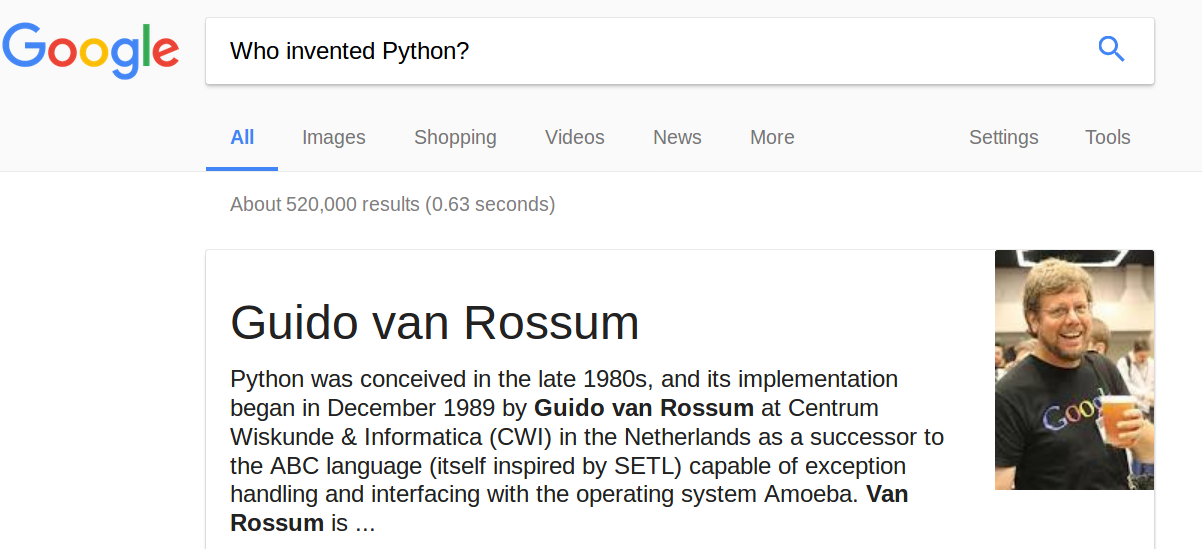
\includegraphics[width=1\linewidth]{./images/Chapitre1/guido_google.png}
	\caption{}
\end{subfigure}

	\begin{subfigure}[b]{0.55\textwidth}
	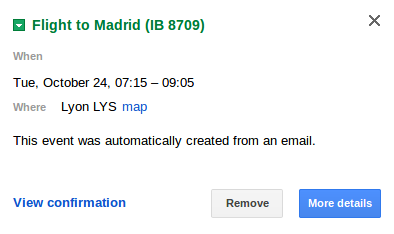
\includegraphics[width=1\linewidth]{./images/Chapitre1/calendar2.png}
	\caption{}
\end{subfigure}
\caption[foo]{(a) While searching \textit{Who invented Python?}, Google recongizes the simple question an directly gives us the answer from Wikipedia. (b) Gmail detects we received an email from an airline and parses it, finds the date, and automatically creates the corresponding event in our calendar.}	
\label{fig:google_nlp}
\end{figure}
%
Indeed, making computers learn,  via theories, algorithms and applications, is the general objective of artificial intelligence research \cite{Sugiyama2015}. Coming from this multi-disciplinary area, Natural Language Processing\footnote{And its more applied branch, text mining or text analysis. While it is sometimes argued that text mining deals with the structured data information extracted from text, I believe both terms considerably overlap nowadays. For ease of readability, in this dissertation we use both terms interchangeably, while preferring Natural Language Processing.} (NLP) is the domain that aims to make machines understand our language\cite{JurafskyM09}. Specifically, speech and text, the latter being the focus of this work.

NLP has developed rapidly \cite{ClarkBook2010} during the last two decades mainly due to the combination of three factors: 
\begin{itemize}
\item The  availability of \textbf{large quantities of freely-accessible textual data}: primarily enabled by the current Web technologies, we are today able to download with a single click the entire content of the English (or other languages) Wikipedia. In the same sense, we can also download thousands of gigabytes of Web crawled data. This information is used to derive knowledge about the text itself, as we will see in the rest of this dissertation. 
\item The \textbf{computational power} at our disposition: from consumer-based computers able to perform parallel computations with considerably large datasets; to on-demand distributed cloud platforms with high performance computing nodes. The latter may be from private providers, e.g., AWS Cloud Service\footnote{\url{https://aws.amazon.com/}}, Microsoft Azure\footnote{\url{https://azure.microsoft.com/en-us/}}, etc; or furnished by public organizations, such as France's Lyon 1 University\footnote{\url{https://p2chpd.univ-lyon1.fr/}} or the National Institute of Nuclear Physics computing centers\footnote{\url{https://cc.in2p3.fr/}}.

\item  The \textbf{large quantity of open-source text mining and data science analysis tools}. Luckily, it is becoming more common for NLP laboratories around the world to make their developments available to the general public, e.g, Stanford University CoreNLP\footnote{\url{https://stanfordnlp.github.io/CoreNLP/}}, Antwerp's University CLiPS Pattern\footnote{\url{http://www.clips.ua.ac.be/pattern}}.
% Paris 7's University Alpage Team Software\footnote{\url{https://www.rocq.inria.fr/alpage-wiki/tiki-index.php?page=Logiciels}}. 
Additionally, large Web companies, such as Facebook\footnote{\url{https://github.com/facebookresearch}} and Google\footnote{\url{https://github.com/google}}, frequently publish their research code and utilities. Lastly, communities of individuals develop libraries that grow to become essential building blocks of several applications and research in the domain. Notably, \texttt{scikit-learn}\footnote{\url{http://scikit-learn.org/}}, a popular data science library implementing several well-known machine learning algorithms. Regarding NLP specifically, two up-to-date libraries stand out:  \texttt{gensim}\footnote{\url{https://radimrehurek.com/gensim/}} and \texttt{spaCy}\footnote{\url{https://spacy.io/}}. These are, for the most part, cross-platform, high performance, optimized, well maintained, documented, easily installable libraries.
% The former specializing on topic modeling and the latter on word's distributional representations.

\end{itemize} 
%
\begin{figure}
\centering
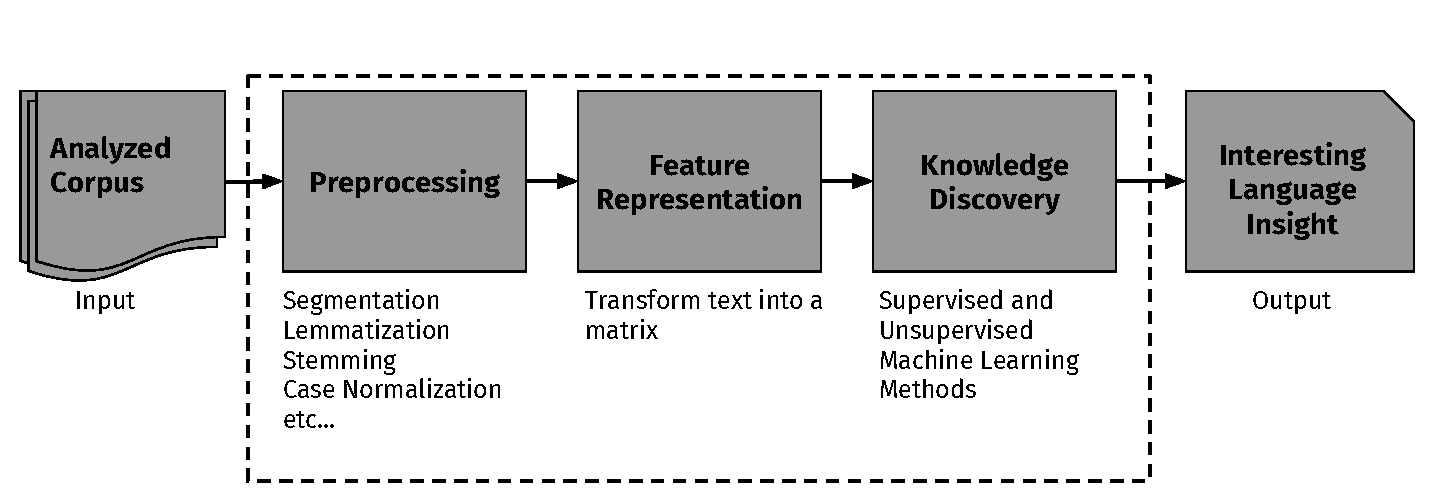
\includegraphics[width=1\linewidth]{./images/Chapitre1/nlp_flow.pdf}
\caption{Typical steps of Natural Language Processing applications.}
\label{fig:nlpflow}
\end{figure}
Solutions to NLP tasks generally follow three steps to achieve their respective goals \cite{mining12Book,JurafskyM09} . First, in \textbf{Preprocessing}, an input corpus is "normalized" so that it will be easier to treat it in the following steps. Secondly, in \textbf{Feature Representation}, a large number of features is extracted from the preprocessed text. Thirdly, in \textbf{Knowledge Discovery},  a machine learning or rule-based (less common nowadays) technique is used to  learn a model able to provide an interesting insight within the existing data as well as on new future instances. The output of said system is usually the model or the language knowledge that reveals an interesting piece of information contained in the input corpus. We can see in Figure \ref{fig:nlpflow}  the typical steps of a NLP system. 

Natural Language Processing is used today for several practical applications. From the elementary tasks that aim to extract linguistic features directly from the text, to more applied systems that employ said features to solve challenging problems. For example, as elementary tasks there is Part-of-Speech (PoS) tagging and Named Entity Recognition (NER). The former, PoS tagging, aims to determine a syntactic class (part of speech) for each word in a corpus \cite{JurafskyM09}. The latter, NER, determines if a proper noun is a place, a person, an organization or any other type of entity required by the final domain and application \cite{nadeau2007survey} . An intermediate task, Word Sense Induction and Disambiguation (WSI/WSD) determines and assigns the semantic meaning of a given word according to its context \cite{ClarkBook2010}.


More complex tasks that generally employ one or more of the aforementioned techniques in order to get more descriptive features from the text and thus get us closer to understand what is being discussed. As an example,  sentiment analysis which ultimate goal of this task is to determine the positiveness or negativeness (or neutrality) of an opinion expressed in a text \cite{liu2012survey}. In this case, it would be useful to know what words express a ``sentiment'': usually adjectives, categorized via PoS tagging; it would be informative to know what (or about who) we are talking about, with NER tagging; as well as the specific context of the words that are being used in the opinion, via WSI/WSD. 



\section{Challenges and Contributions}
There are several research challenges that arise from the choices taken in each one of the steps comprising the NLP system's flow (Figure \ref{fig:nlpflow}).
 In this thesis, we particularly focus on three challenges arising in both the Feature Representation and Knowledge Discovery phases:
\begin{itemize}
 \item \textbf{Feature Representation:}
	 \begin{enumerate}
	 \item  Modeling, extracting, and storing different types of linguistic features from raw text. 
	 \item Dealing with the sparsity inherent to text data while successfully combining the different available text features.
	
	 \end{enumerate}
 \item \textbf{Knowledge Discovery:}
 	\begin{enumerate}
 	\item[3.] Finding relations  between words and then leveraging them in order to discover their latent relatedness and be able to solve NLP tasks.
  	\end{enumerate}
\end{itemize}


The contributions that we propose in this work are the following:
\begin{itemize}
\item a structural network-based model to hold heterogeneous linguistic data as well as a tool to extract said data from unstructured text.
\item a network-based algorithm to discover similarity relations between linked words
\item a method to combine heterogeneous representations while at the same time alleviating the sparsity problem common while dealing with text features.
\end{itemize}
These contributions are tested and evaluated using two different NLP semantic tasks: Word Sense Induction and Disambiguation and Named Entity Recognition. We chose these two tasks as they are semantic problems directly benefited by methods  that are able to determine the relatedness among words, which is the case of the techniques we propose. Not less important, we attack these tasks as they are central building blocks of more intricate text analysis systems. Our propositions are built using open source tools and trained/tested using freely accessible corpora. We aim to make our software implementations are  to multi-threaded CPU computers when applicable.


\subsection{Modeling linguistic features}
\paragraph{Challenge}
Representing unstructured text within a model that describes textual units and their corresponding features is a critical step within a NLP process. Textual units -- either words, sentences, paragraphs, documents, etc -- need to be represented by some kind of model that will allow for numerical analyses to be applied. Usually, textual units are represented in a vectorial space, where each dimension represents a feature; or in a graph-like structure, where features link units together. Concerning the features themselves, their selection is often an empirical process determined  by the final goal of the NLP process at hand. Nonetheless,  we have access to several types of linguistic features, each one representing the text from different points of view.  Furthermore, texts usually containing large vocabularies involves the need of an efficient way of storing a corpus and its features. These possibilities entail the following research questions: what type of model can we employ to represent a corpus through a set of heterogeneous features, extracted from itself, while keeping record of the relationships between textual units? How can we organize and store this model as simply and efficiently possible? These questions allow us to properly constitute a linguistic resource adapted to solve NLP tasks while having an heterogeneous description of the textual units\footnote{In this work we focus on words. As such, the rest of this dissertation deals with the representation of words.}


\paragraph{Contribution}
Determining which kind of structure will hold textual features as well as 
An annotated parsed dump of the English Wikipedia. In this parse we focus  onto the syntactical characteristics of words: aside from the classical Part-of-Speech (PoS) tags and dependency parsing relations, we provide the full constituent parse branch for each word in a succinct way.  



\subsection{Combining features and dealing with sparsity}
\paragraph{Challenge}

 We explore multimedia fusion techniques to complement the features hold by the network. Specifically, we focus on solving named entity recognition and word sense induction and disambiguation by applying feature-combination methods that have already shown their efficiency in the multimedia analysis domain.  Our results show that the combination of textual features indeed improves the performance compared to single feature representations and trivial features concatenation. Even more, we experiment with background information from open text sources to further improve the performance of our models. Finally, we also present an analysis on the behavior of features according to different types of senses and entity classes.



\paragraph{Contribution}
\newpage
\subsection{Leveraging the network to find semantic relatedness}
\paragraph{Challenge}
An algorithm that leverages  the structure of the network in order to solve word sense induction and disambiguation. Our proposed method takes into consideration the "real-world" characteristics of the graph to group similar senses and then assign them to target words. We  improve the overall performance compared to other similar graph-based techniques.

\paragraph{Contribution}






\begin{figure}
\centering
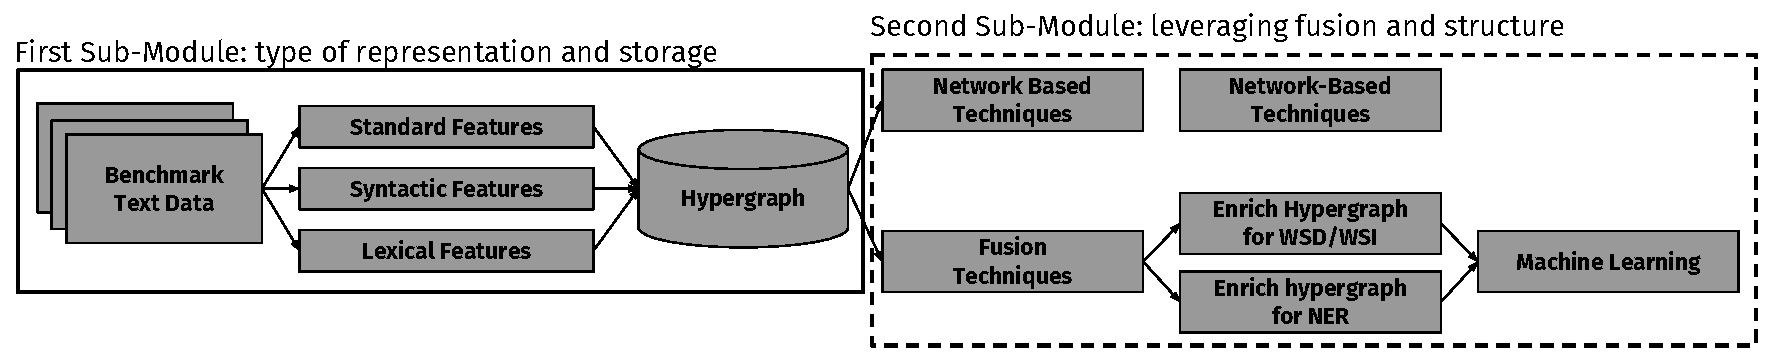
\includegraphics[width=1\linewidth]{./images/Chapitre1/main_diag2.pdf}
\caption{Modular description of this dissertation}
\label{fig:maindiag}
\end{figure}





%\section{Contributions}
%Having cited the disadvantages of current language representations and applications, we set out to fill the gaps with our own propositions. First, in order to have a dataset to test and work with, we parsed and stored the English Wikipedia taking into account largely-ignored syntactic information. Secondly, we fitted our linguistic network to a sample of the parsed Wikipedia corpus. Thirdly, we proposed an algorithm to solve word sense induction and disambiguation by leveraging the network's structure. Finally, we present a method that combines textual features to solve both named entity recognition and again word sense induction and disambiguation. More concisely, we make the following contributions in this dissertation:

Figure \ref{fig:challenges_contribs} synthesizes the concerned NLP process-flow stages, their existing challenges and their related contributions, and the tasks used to validate our contributions. We briefly introduce our contributions and their context in the following subsection.

\begin{figure*}
\centering
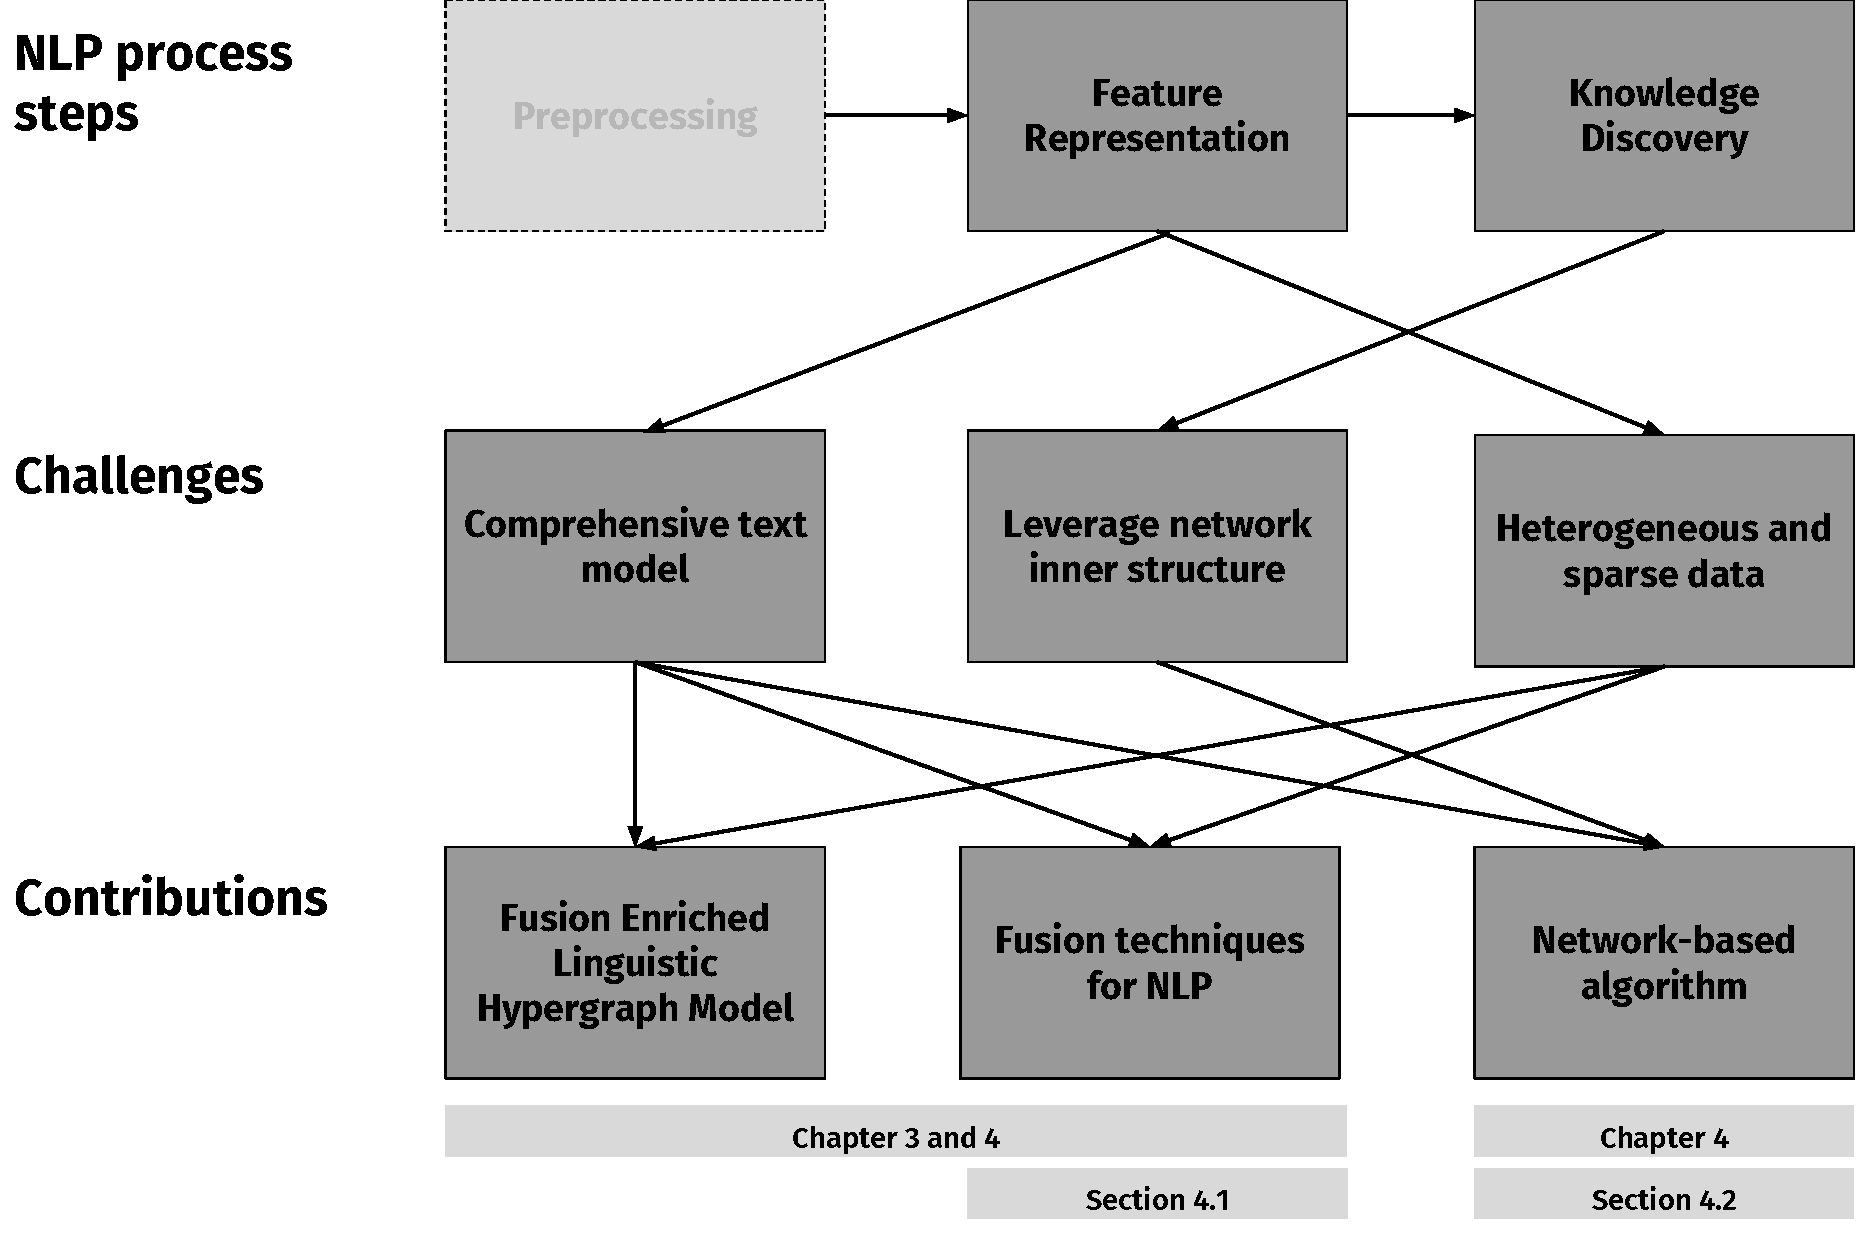
\includegraphics[width=1\linewidth]{./images/Chapitre1/challenges_contribs.pdf}
\caption{}
\label{fig:challenges_contribs}
\end{figure*}
\section{Structure of the Dissertation}
The remainder of this thesis is structured as follows:
\paragraph{Chapter \ref{chap:backgnd}} This chapter has a detailed overview about the first four axes of this thesis: how we can represent words from a lexical, syntactic and semantic point of view, then, how we find relatedness among words based on  the distributional hypothesis, and how we link both words and features together in a language network to discover their structure and to extract useful knowledge. 
%
%Afterwards, we present how these features can be combined to improve the results of single-feature based solutions. 
Afterwards, we detail the machine learning methods used to solve the NLP tasks. Finally, we present the two NLP tasks we solve using our propositions: Word Sense Induction and Disambiguation (WSI/WSD) and Named Entity Recognition (NER).
\paragraph{Chapter \ref{chap:related_wk}} We discuss previous work related to the main contribution of this work, linguistic networks. We cover the previous work specific to each task in its corresponding chapter.

\paragraph{Chapter \ref{chap:ling_net}} We present and define a novel structure to hold language information: the hypergraph linguistic model.  We discuss its characteristics and the intuitions behind its conception: the hypergraph choice,the role of nodes and edges, the type of features stored, the advantages it present in terms of accessing and manipulating the data. In the following chapters, we address the applications that leverage the properties of the structure proposed.

\paragraph{Chapter \ref{chap:wsd}} In this chapter, we present an algorithm that exploits the structure of the network, i.e., the connections between nodes. Namely, we derive senses from a test corpus by finding related words connected to a single main node. We test the linguistic and lexical features and discuss about its qualities. Our results improve on the performance of similar propositions from the literature. We study the combination of features using multimedia fusion techniques in the next chapter.

\paragraph{Chapter \ref{chap:fusion}} We explore the application of multimedia fusion techniques using linguistic features to solve NLP tasks. Briefly, fusion techniques may consist on trivially concatenating feature columns or a combination that aims to transfer relatedness information from one representation to a second one. We experiment with these methods on three datasets for named entity recognition and one dataset for word sense induction and disambiguation. Indeed, we show that using certain configurations of fusion techniques can lead to improvements over single-feature and trivial-concatenation representation matrices. Furthermore, we explore the contribution from each representation kind to each sense and class in each task respectively.
\paragraph{Chapter \ref{chap:dump}} This chapter describes the process of parsing and storing an English Wikipedia Syntactical Dump. We use open source tools on freely available data to generate a software that is able to extract lexical and syntactic data from a given corpus.We thus create and publicly release a syntactically annotated version of the English Wikipedia containing often-neglected information, stored in a format that facilitates its manipulation. 

\paragraph{Chapter \ref{chap:conclusions}} We conclude this dissertation and present possible avenues for future work.

